\chapter{Molecular Library Generator and Virtual High-Throughput Screening Framework}
	
%\chapter{Rational Design Framework for Accelerating the Discovery of Materials}

The discovery of new compounds, materials, and chemical reactions with exceptional properties is the key to progress in chemistry. This process can be dramatically accelerated by means of the virtual high-throughput screening of large-scale candidate libraries. This approach has been extensively used for many years in the drug discovery community and has more recently been applied to the search for energy materials. The key challenge is that chemical space is practically infinite, and any approach to survey it or enumerate certain of its domains has to address the problem of combinatorial complexity.

Therefore, we have developed a general-purpose suite, \chemlg , a generator for compound and material candidate libraries. In this chapter, we primarily discuss the algorithms implemented in \chemlg, and give examples of its successful application in various domains. We also briefly discuss the other three software packages in our group's software ecosystem, \chemhtps, \chembddb, and \chemml.

I am the primary developer of \chemlg\ code. The code \chemhtps\ was co-developed with William Evangelista. The developers of \chembddb\ are Aditya Sonpal and Shirish Sivaraj, whereas the primary developer of \chemml\ is Mojtaba Haghighatlari. 

\section{Introduction}

A prerequisite for the high-throughput exploration of chemical space is access to suitable, large-scale screening libraries. The key for a successful library generation approach is to balance the ambition for a systematic and exhaustive enumeration of the combinatorial search space, with the need for an efficient and responsive scheme. The generation of combinatorially exhaustive libraries is relatively straightforward, but it rapidly becomes impractical for screening purposes due to its exponential growth. For instance, the largest small-molecule library, GDB-17, contains 166.4 billion molecules, which were generated using only up to 17 atoms (C, N, O, S, and halogens) \cite{Reymond2012}. Most currently available codes are thus limited to generating small, drug-like molecules. 

\chemlg\ extends and generalizes the molecular library generation to identify lead candidates in various applications such as functional polymers, optoelectronics, and catalysis. It offers a multitude of options to customize and restrict the scope of the enumerated chemical space and thus tailor it for the demands of specific applications. To streamline the non-combinatorial exploration of chemical space, we incorporate genetic algorithms into the framework. Genetic algorithms have shown to be efficient in optimizing chemical structures and generating useful compounds for different target applications. In addition to implementing smarter algorithms, we also focus on the ease of use, workflow, and code integration to make this technology more accessible to the community. 


\section{Methodology}

There are two different approaches for enumeration of compound space: product-based approach and reaction-based approach. The former one is based on the application of Markush structures, which expands the library by attaching the functional groups to various sites on the scaffold whereas the latter approach is based on chemical transformation [4]. Combinatorial libraries can be obtained by using three different algorithms: the first is the ‘grow’ algorithm where the growth in the molecule starts from a seed point, second is the ‘fragment-link’ algorithm and the third algorithm is the sampling approach where the growth of the molecules is based on random selection [5]. In our generator, we use the ‘fragment-link’ method which follows a reaction transform approach. The reaction can be obtained by two methods: first method is the reshuffling of the SMILES strings and the second method follows an actual reaction scheme. Both of these methods are discussed in the following subsections. 

\subsection{SMILES Rearrangement}

SMILES, which stands for simplified molecular-input line-entry system, is a string notation for describing the structure of chemical species \cite{Anderson1987}. It is a widely used notation as it is human readable and can be imported by most molecule editors for molecular visualization. In the SMILES rearrangement method, the SMILES of the linking molecules is written such that the linking atoms are positioned at the extreme end of the string. The linkage can then be obtained by directly combining the SMILES strings. A schematic representation of this method is shown in the Fig.\ \ref{fig:validation}. In this method, it is not necessary to specify reaction sites or have to use any reaction algorithm. This way of linkage can generate all possible combinatorial structures. 

\begin{figure}[htbp] 
	\centering
	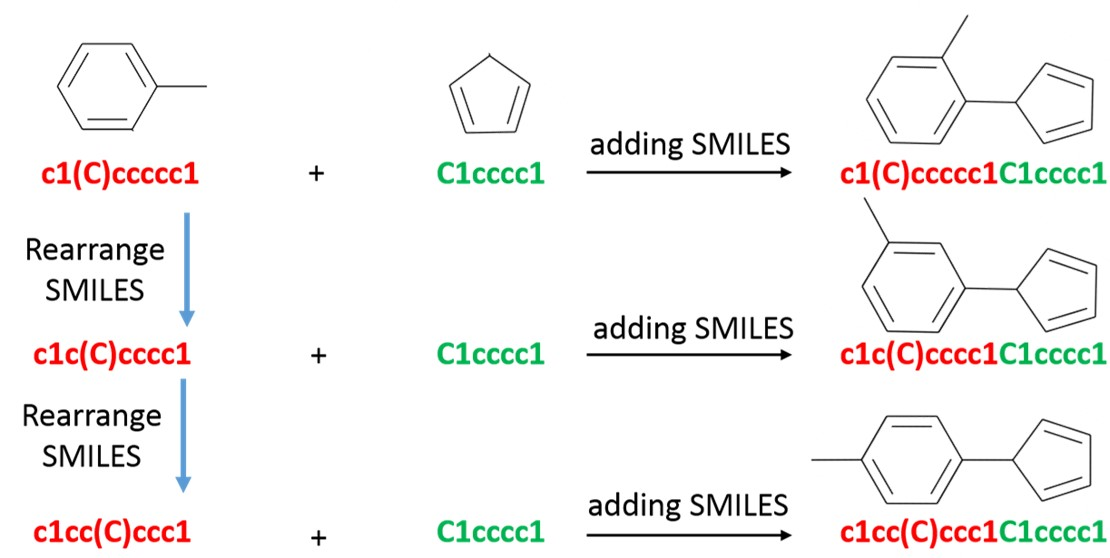
\includegraphics[width=0.9\textwidth]{Chapter-4/Figures/SMILES_link.jpg}
	\caption{Fragment linkage based on SMILES rearrangement.} 
	\label{fig:SMILES_link} 
\end{figure}  

We developed a code to represent the SMILES of a molecule with all possible string notations in which the chemical handles are positioned on the extremes. This method is extremely powerful as it can produce a large molecular library spontaneously. Further, this method is more suited for the generation of polymer libraries. We apply this method to generate a library of polyimides for the exploration of high-refractive-index polymers discussed in Chapter 5. However, there are a few limitations to this approach. For example, a large number of duplicates will be generated in the process and the removal of duplicates will be computationally expensive. Additionally, narrowing the chemical space will be difficult as applying constraints on string notations is challenging. Further, the generation of fused molecules is not possible using this approach.

\subsection{Fragment Link and Fusion}

Fragment link or fusion of fragments is performed by casting into a reactor. The reactor in \chemlg\ takes the fragments as arguments along with combination type and generates a linked or fused molecule. A schematic representation for the link and fusion of molecules is shown in the Fig.\ \ref{fig:link+fusion}. In this scheme, the reaction sites on the fragments are denoted as X. In case of linking, once the reaction occurs, there is a bond formed between the fragments and X is removed. While, in fusion, the molecules lose two carbons and a hydrogen along with X.

\begin{figure}[htbp] 
	\centering
	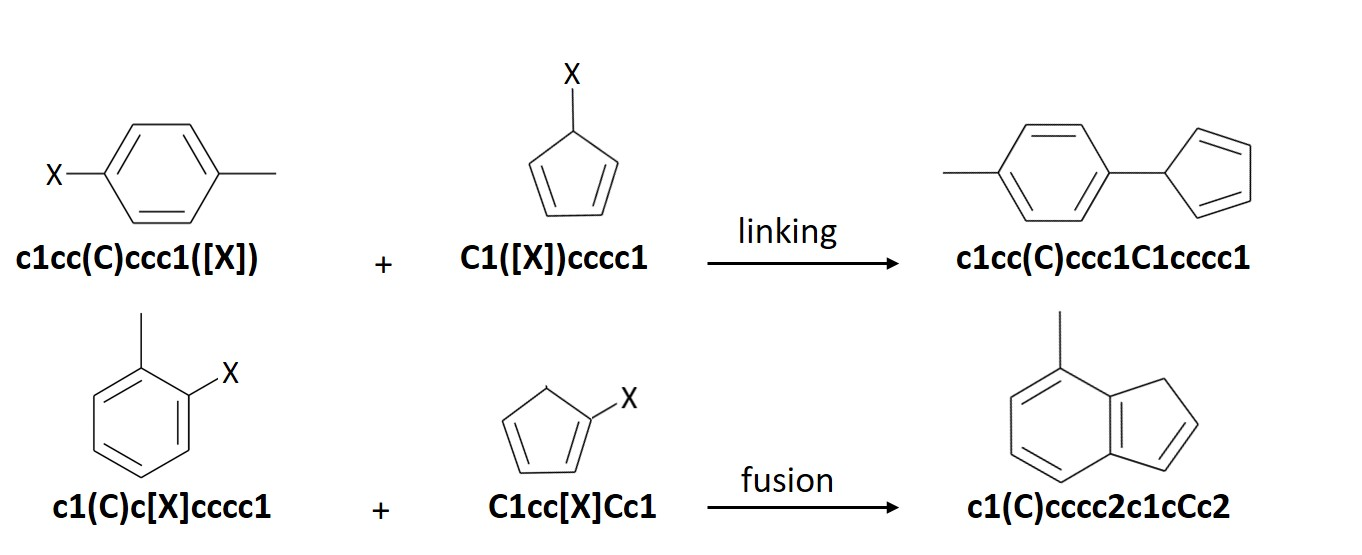
\includegraphics[width=0.9\textwidth]{Chapter-4/Figures/link+fusion.jpg}
	\caption{Schematic for the link and fusion of molecules in \chemlg.} 
	\label{fig:link+fusion} 
\end{figure}  

\section{Generation Constraints}

We find that instead of exploring a limited chemical domain exhaustively, it is often more useful to bias the search in directions where candidates are most promising and synthetically viable. In our development of \chemlg\ , we have thus augmented the combinatorial schemes by a number of `smart' modules that make use of additional input. To address the concern that virtual candidates may not be accessible or desirable (\eg  from a synthetic perspective), we have introduced a constrained-growth scheme that continually prunes the generation process. In this scheme, molecules are rejected at every generation to constrain the growth as shown in the Fig.\ \ref{fig:constrained}. It accepts user-defined constraints, \eg  to exclude certain structural patterns or substructures, fingerprint matching, building block combinations, or sequences; to limit size or chemical makeup; or to enforce symmetries or other rules (\eg  Lipinski's rule).
%\begin{enumerate}
%	\item Include building blocks
%	\item Min and max no. of bonds 
%	\item Min and max no. of atoms 
%	\item Min and max mol. weight 
%	\item Min and max no. of rings 
%	\item Min and max no. of aromatic rings
%	\item Min and max no. of non-aromatic rings
%	\item Min and max no. of single bonds 
%	\item Min and max no. of double bonds
%	\item Min and max no. of triple bonds
%	\item Max no. of specific atoms
%	\item Lipinski's rule
%	\item Fingerprint matching
%	\item Substructure
%	\item Substructure exclusion
%\end{enumerate}

\begin{figure}[htbp] 
	\centering
	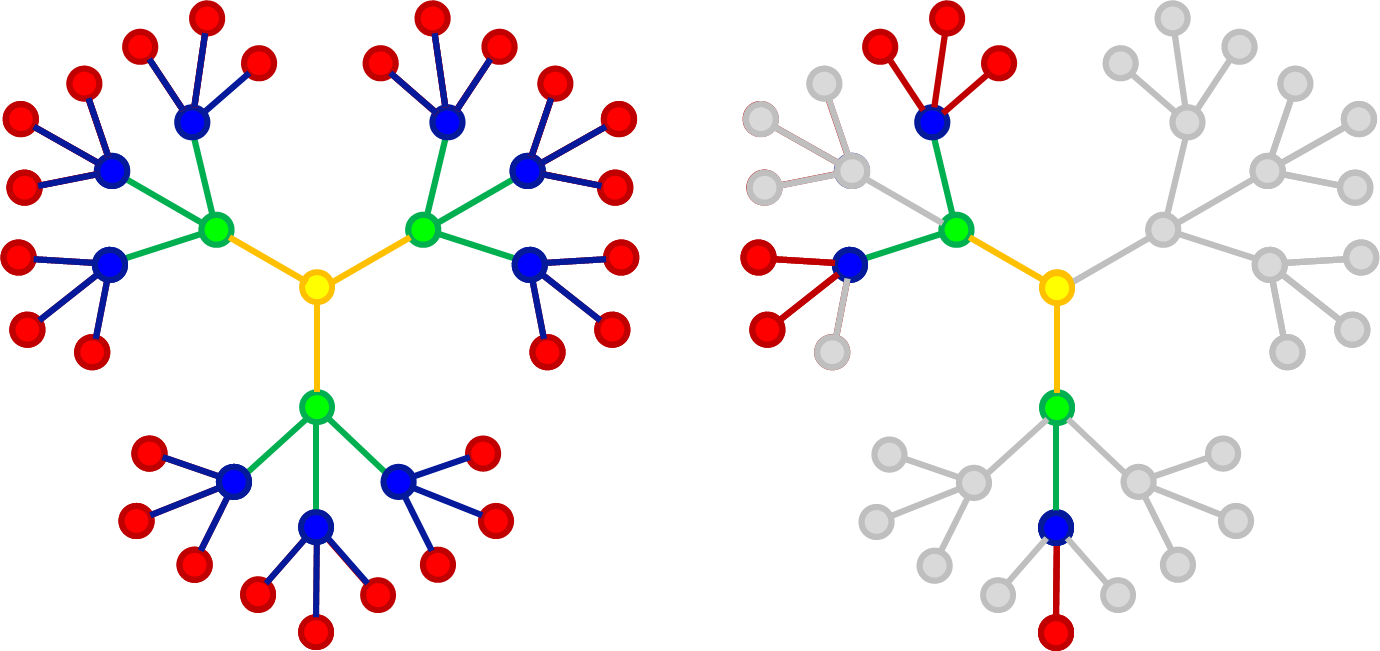
\includegraphics[width=0.9\textwidth]{Chapter-4/Figures/constrained.png}
	\caption{Schematic for constrained growth of molecular library. The left scheme shows an exhaustive enumeration, whereas the right scheme represents a targeted enumeration.} 
	\label{fig:constrained} 
\end{figure}  

\section{Smart Algorithm}
Even applying above mentioned generation constraints might lead to a large number of unwanted molecules in the library. We need to only target the molecules that are of interest and discard the rest. Application of smart algorithms can narrow down the chemical space to a more specified regions. A schematic for the pruning of molecular libraries is shown in Fig.\ \ref{fig:smart_algo}. \chemlg's genetic algorithm module allows us to optimize candidate pools and the chemical structures they contain for specific target applications. 

\begin{figure}[htbp] 
	\centering
	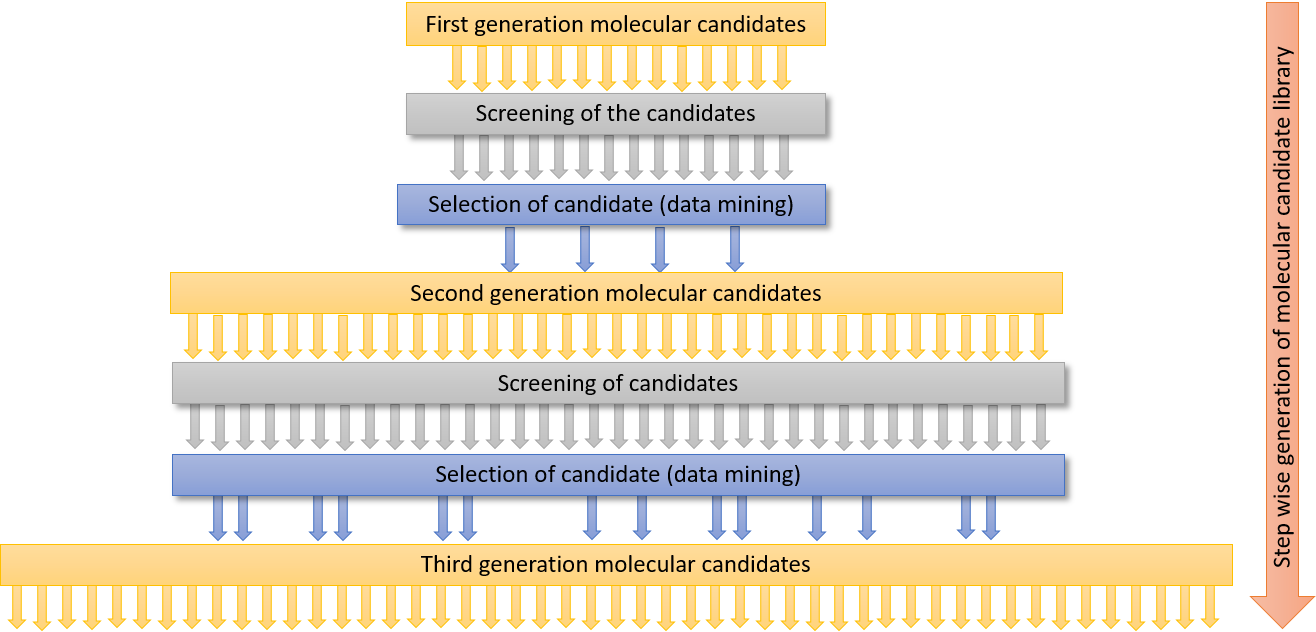
\includegraphics[width=0.9\textwidth]{Chapter-4/Figures/smart_algo.png}
	\caption{Pruning of molecular library at every generation by use of smart algorithms.} 
	\label{fig:smart_algo} 
\end{figure}  

We employ an on-the-fly prescreening through rapid candidate assessment \via\ DFT, MD, or data-derived prediction models. These models also serve as fitness functions in \chemlg 's genetic algorithm module, which allows us to optimize candidate pools and the chemical structures they contain for specific target applications. In genetic algorithm approach, at every generation of molecular library, best candidates are retained and certain operations are performed to generate new promising candidates. These operations include crossover and mutation (see Fig.\ \ref{fig:GA}). In the crossover operation, the structures from top candidates are split and exchanged with each other. Whereas in mutation, randomly selected substructure is replaced with other building blocks from the initial list. Following this scheme for several generations will result in a library that is tailored for a targeted application. As an example, this scheme is applied to create a library of molecules with similar structure to a targeted molecule with fingerprint matching as fitness function (see Fig.\ \ref{fig:GA_example}). We observe that at every generation we obtain molecules that match better to the target molecule. 


\begin{figure}[htbp] 
	\centering
	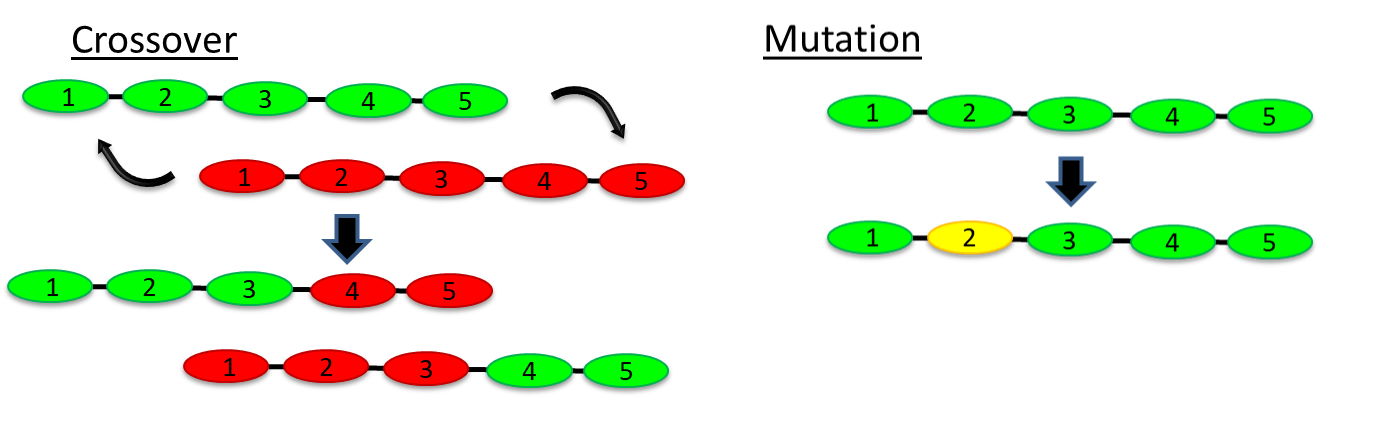
\includegraphics[width=0.9\textwidth]{Chapter-4/Figures/GA.png}
	\caption{Genetic algorithm operations: crossover and mutation.} 
	\label{fig:GA} 
\end{figure}  


\begin{figure}[htbp] 
	\centering
	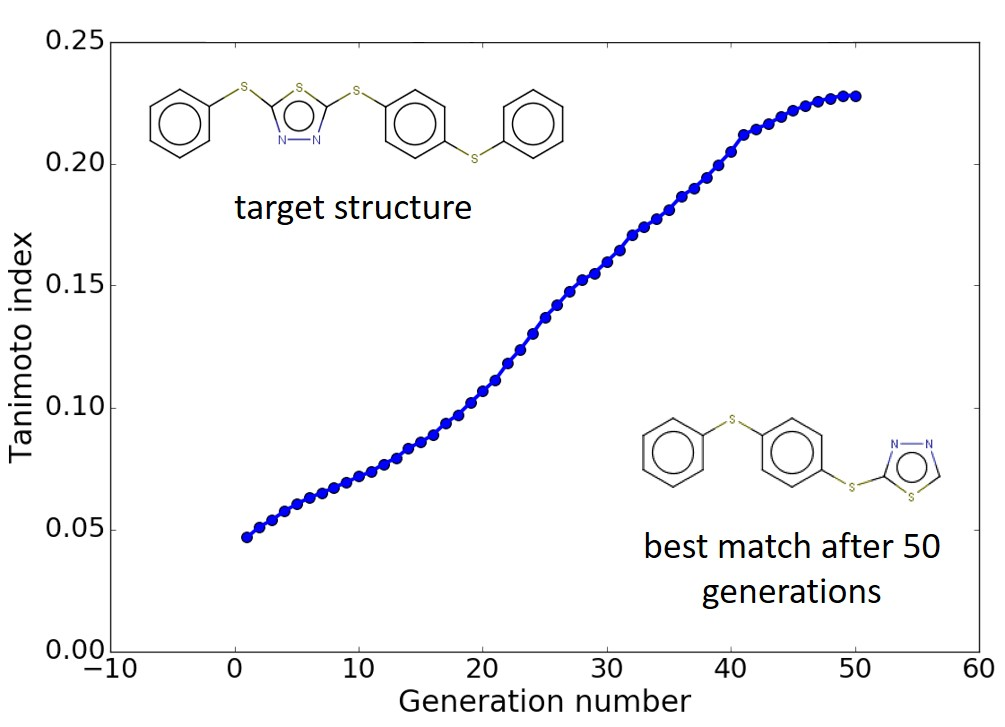
\includegraphics[width=0.75\textwidth]{Chapter-4/Figures/GA_example.jpg}
	\caption{Implementation of genetic algorithm to find similar structures.} 
	\label{fig:GA_example} 
\end{figure}  


\chemlg 's `smart' modules can thus facilitate self-regulating growth of the candidate libraries and ultimately a self-optimizing traversal of chemical space. It offers options for the various approaches mentioned above to provide the most suitable solution for different problem settings. We have successfully employed \chemlg\ to produce screening libraries for a number of application projects.


\section{Parallel Implementation of \chemlg}

An important feature of \chemlg\ is that the code is massively parallel. The parallelization is obtained using MPI4Py library and it is implemented at various levels to accelerate the library generation process (see Fig.\ \ref{fig:ChemLG_parallel}). This allows us to create a library of millions of molecules in just a few seconds. The bottleneck step is the removal of duplicates at every level. There are several algorithms for efficient removal of duplicates, but they are designed to run in a serial fashion. Parallelizing these algorithms is not efficient as there is significant communication overhead in the process. For efficiently scraping duplicated in molecular library, we exploit the fact that no two molecules with different molecular weights are same. We group the molecules based on their molecular weights by keeping tags and scatter the groups to different processors for duplicates removal. This process is efficient as it involves no communication between the processors. The speedup and parallel efficiency of the code for the generation of a million candidates is shown in Fig.\ \ref{fig:ChemLG_performance}. The performance of \chemlg\ scales very well with increasing number of processors. Due to a high-level of parallelization, \chemlg\ performs well on a high performance computing (HPC) platform. This is helpful as it integrates well with \chemhtps\ infrastructure, where the molecular library can be generated and readily applied for HTPS.

\begin{figure}[htbp]
	\centering
	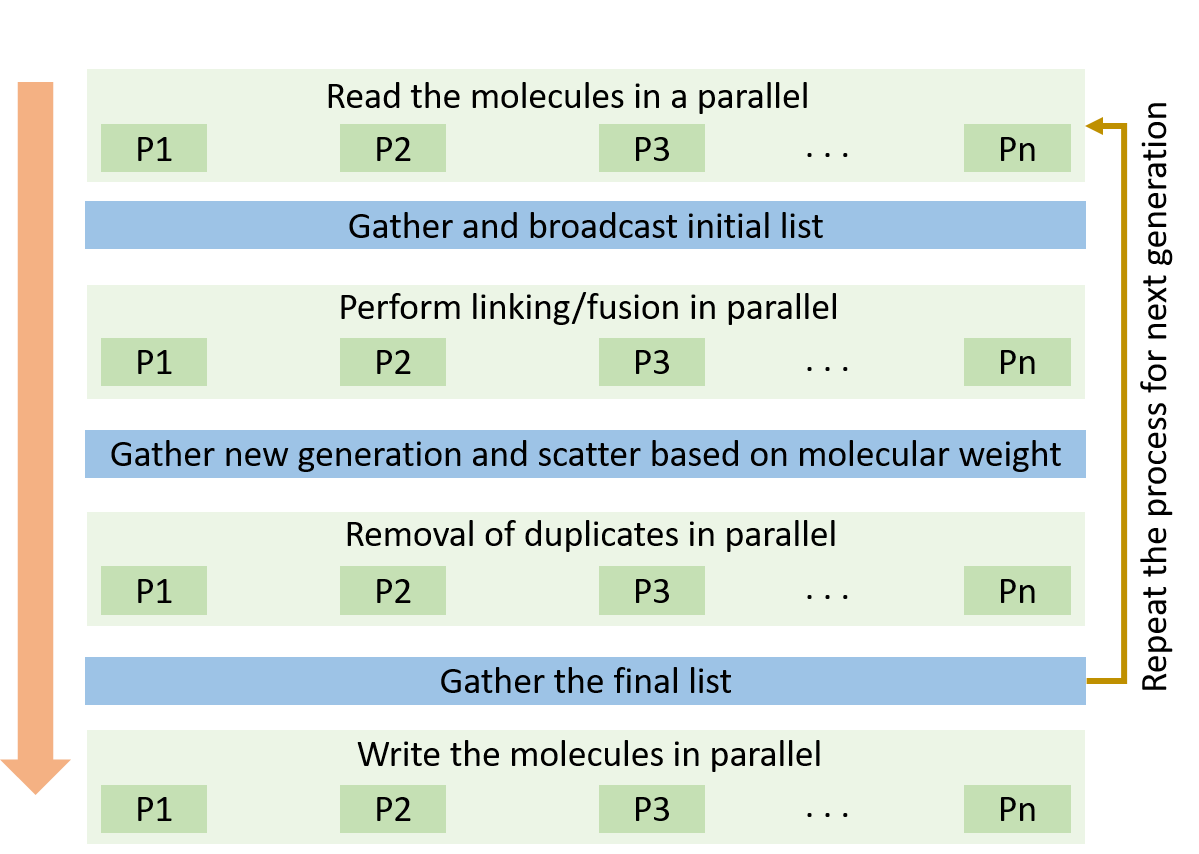
\includegraphics[width=0.75\textwidth]{Chapter-4/Figures/ChemLG_parallel.png}
	\caption{Levels of parallelization in \chemlg\  package.} 
	\label{fig:ChemLG_parallel} 
\end{figure}  

\begin{figure}[htbp] 
	\centering
	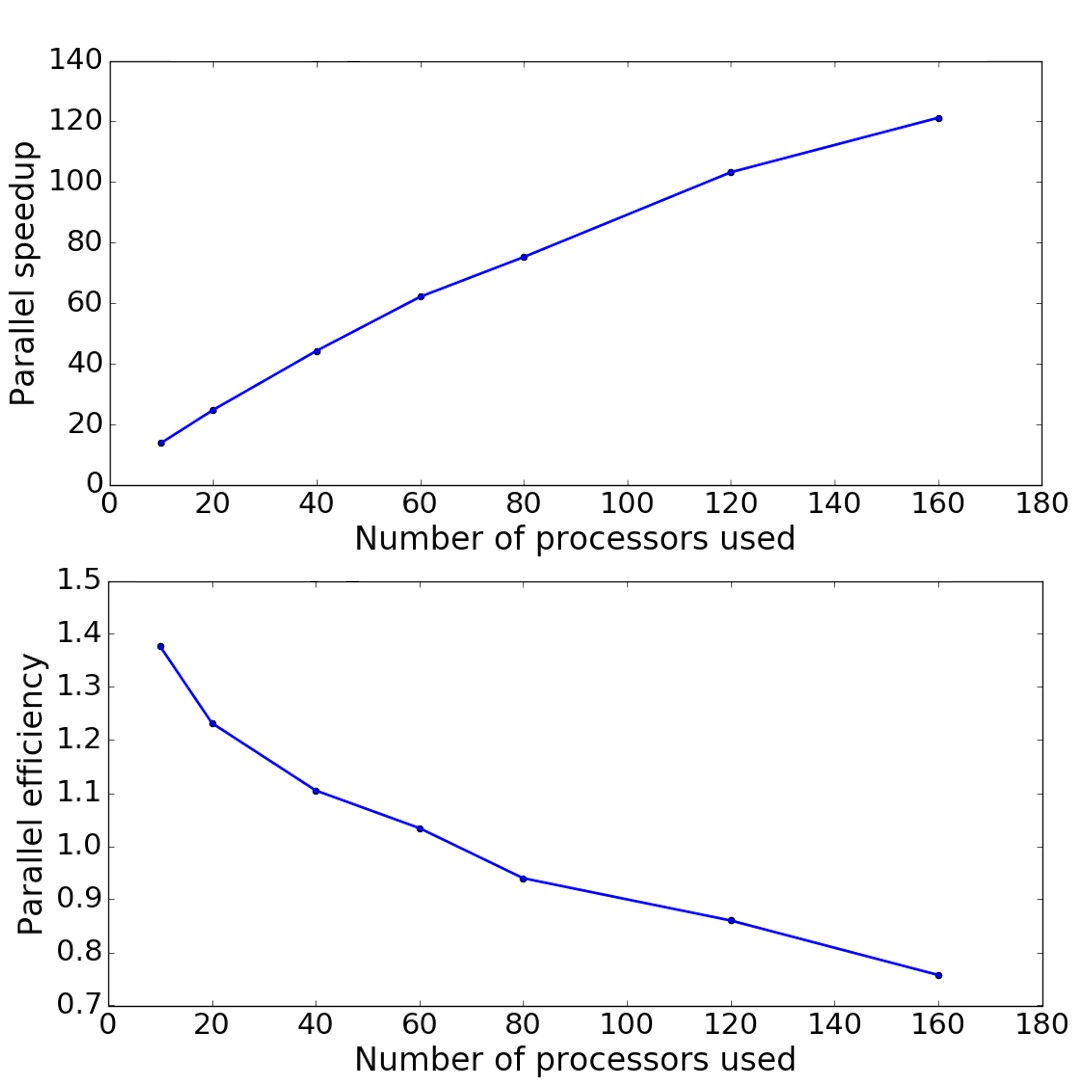
\includegraphics[width=0.7\textwidth]{Chapter-4/Figures/ChemLG_performance.jpg}
	\caption{Parallel speedup and efficiency observed in \chemlg\ package.} 
	\label{fig:ChemLG_performance} 
\end{figure}  

\section{Example Applications of \chemlg}
\label{subsec:chemlg_app}

\chemlg\ has been successfully applied in various applications. In the current dissertation, it is applied to make a library of polyimides and small organic molecules for the exploration of chemical systems with high RI values. Further details of these two libraries are discussed chapter 5 and chapter 6, respectively.

The generator was also used for creating a library of polyesters in a quest to design polymers with superior degradation behavior. We found that the activation energy for the degradation of polyesters is dependent on the functional groups that are attached to the $\beta$-carbon of the ester bond. This results motivated us to generate a library functional groups that can ba attached to $\beta$-carbon. This project is being led by Vigneshwar Kumaran Sudalayandi Rajeswari. 
  
In another project, internship work at ExxonMobil Chemical Company, \chemlg\ was used to create a library of novel polyolefins \cite{Afzal2018d}. The library was built by linking saturated carbon atoms in a combinatorial fashion. We used methane, ethane, and butane as the building blocks while considering all the hydrogens as connection sites. Using these rules, the library was built until three generations, which resulted in 275 monomer structures. These monomers were used to build corresponding oligomers and subsequently screened them in a virtual high-throughput fashion to evaluate their coil dimensions.

\chemlg\ has also been instrumental in formulating chemical libraries for compounds with application as deep eutectic solvents (DES) and photosensitizing (PS) catalysts. Candidate compounds were obtained by relying on a common molecular structure, for e.g., alcohols and amides as hydrogen bond donors in DES systems, and corroles and porphyrins for PS systems. Different building blocks were attached to these molecular backbones at desired linking sites to get hundreds of thousands of candidate molecules in each case. These libraries are part of a strategy to exhaustively access chemical spaces of interest for these applications. Yudhajit Pal is taking a lead on these two projects.

\section{Other Parts of Group's Cyberinfrastructure}

\subsection{Virtual High-Throughput Screening Infrastructure}
\label{subsec:chemhtps}

A prerequisite for conducting computational high-throughput screening studies is a software infrastructure that can facilitate the execution of thousands or even millions of modeling calculations. For this task, we have been developing the \chemhtps\ program suite. A schematic for a typical use of HTPS is represented in Fig.\ \ref{fig:screen_pipe}. \chemhtps\ is designed to streamline and automatize the setup of project environments and directory structures, the generation of job pools based on user-defined candidate libraries (\eg  from \chemlg ) and modeling protocols, their submission to available hardware in an orderly and load-balanced fashion, job monitoring, error handling, as well as the parsing and bookkeeping of returning results. These processes follow generalized workflow templates that we have been developing from abstraction in the course of different application projects. It currently supports the ORCA \cite{Neese2012}, Q-Chem \cite{Shao2014}, and GROMACS \cite{ABRAHAM201519} modeling packages, and bindings to other quantum chemistry, molecular dynamics, and solid state physics codes are planned for the future. Given the required user input for the candidate library and modeling protocols, we can now set up and launch a high-throughput \insilico\ screening project like the Clean Energy Project \cite{Hachmann2011,Olivares-Amaya2011,Amador-Bedolla2013,Hachmann2014,Pyzer-Knapp2015,Lopez2016} from scratch in a few minutes, which is a dramatic reduction from its original lead time of several months. We have been using \chemhtps\ in a number of studies, searches for new high RI polymers, deep eutectic solvents for supercapacitors and battery electrolytes, molecular hydrolysis catalysts for solar water splitting and fuel cells, doped and defect nanographene anode materials for lithium ion batteries, polyvinyl-based biodegradable polymers for biomedical plastics, liquid organic hydrogen carriers for the hydrogen economy, and organic semiconductors for photovoltaics and other applications \cite{Hachmann2011,Olivares-Amaya2011,Amador-Bedolla2013,Hachmann2014,Lopez2016,Afzal2018a,yujie_msthesis,chingyen_msthesis,manprep}. In the case of high RI polymers, we apply this framework to automate the calculations for the polarizability (see Fig.\ \ref{fig:workflow}) and packing density. Contributions to \chemhtps\ were made by William Evangelista. 

\begin{figure}[htbp]
	\centering
	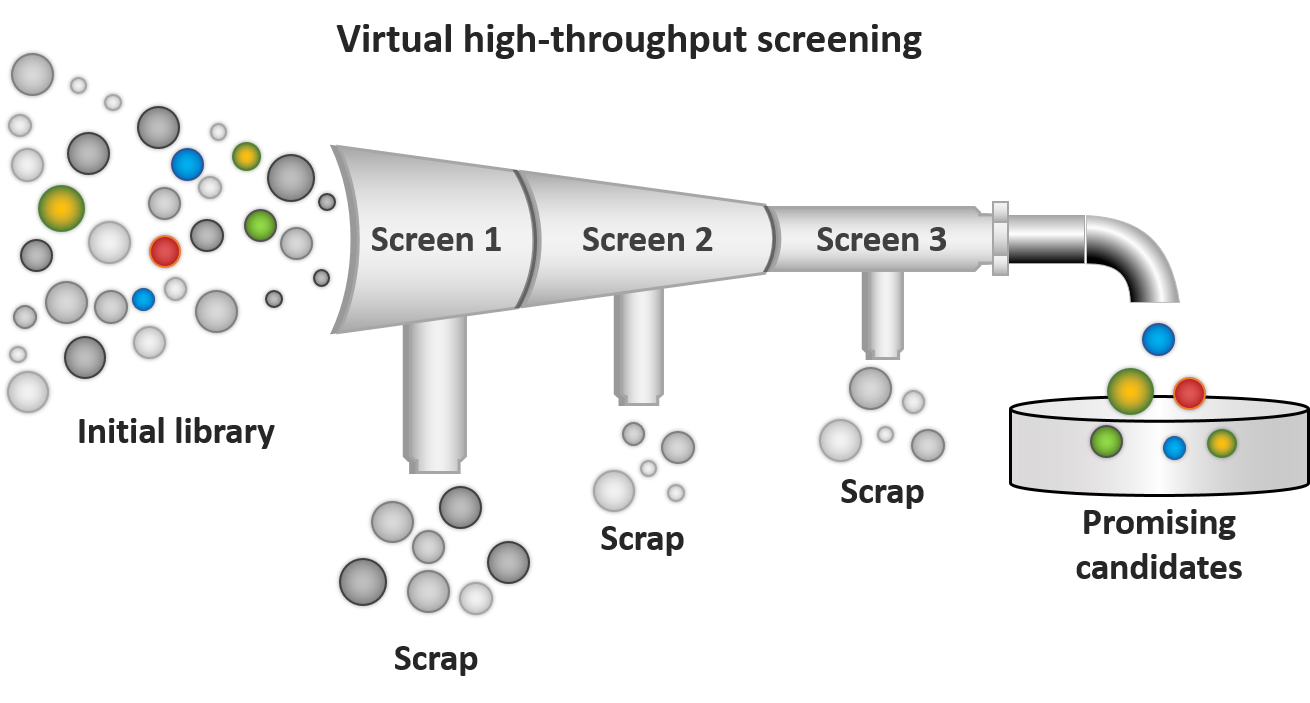
\includegraphics[width=0.9\textwidth]{Chapter-4/Figures/screen_pipe.png}
	\caption{Schematic for the screening of a library of molecules to identify promising candidates. At every level of screening, a higher level of theory is applied while narrowing down the chemical space.} 
	\label{fig:screen_pipe} 
\end{figure}  

\begin{figure}[htbp]
	\centering
	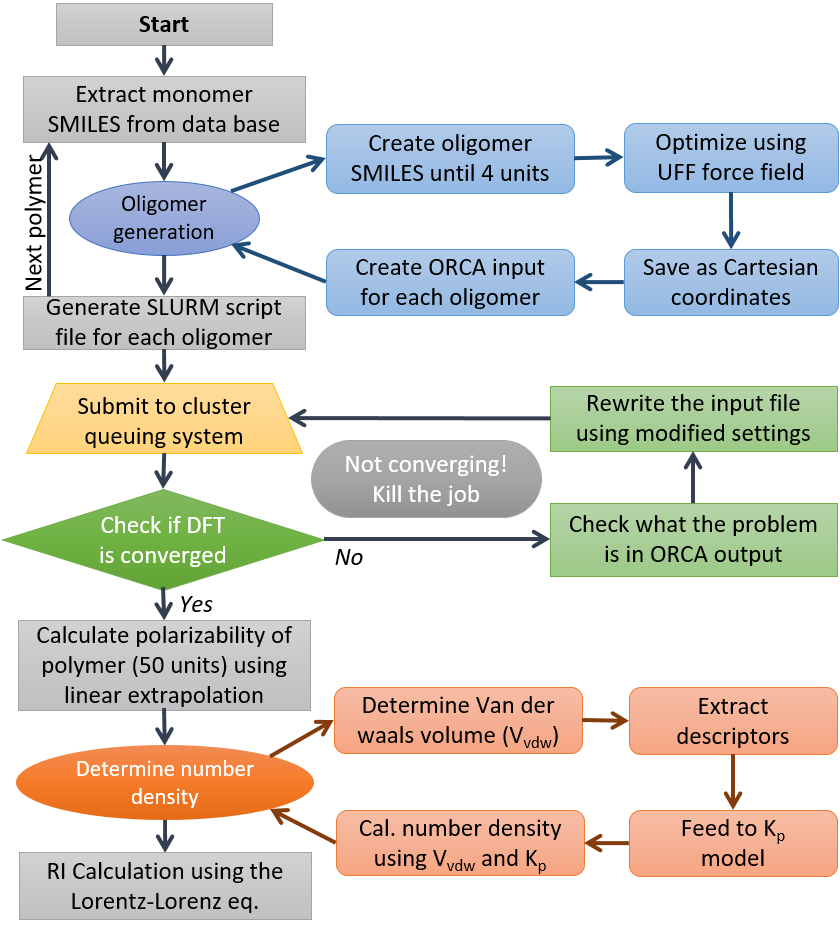
\includegraphics[width=0.7\textwidth]{Chapter-4/Figures/workflow.png}
	\caption{Work-flow implemented for the automation of polarizability values of candidate libraries.} 
	\label{fig:workflow} 
\end{figure}  


\subsection{Database Infrastructure}
\label{subsec:chembddb}
The use of modern database technology is of particular importance in the context of data-intensive research. Despite their great utility and despite being essential for projects that accumulate large data sets, databases are still rarely featured in chemical research. Our group is developing the \chembddb\ code to simplify and streamline the use of databases and thus make them more accessible to non-expert users in the chemistry community. \chembddb\ provides an automated database setup, a data model template that can readily be customized, and the necessary tools to access and manipulate the database. 
As in \chemhtps\ , we have been developing the corresponding workflows by abstracting our experience from real-life application projects with flexibility and reusability in mind. All the data generated from the virtual high-throughput screening of high RI polymers is incorporated into a database using \chembddb. Screenshots of the database are shown in Fig.\ \ref{fig:chembddb_screenshot}, which were provided by Shirish Sivaraj. 

Developers of \chembddb\ are Aditya Sonpal, Shirish Sivaraj and Supriya Agrawal. 

\begin{figure}[htbp]
	\centering
	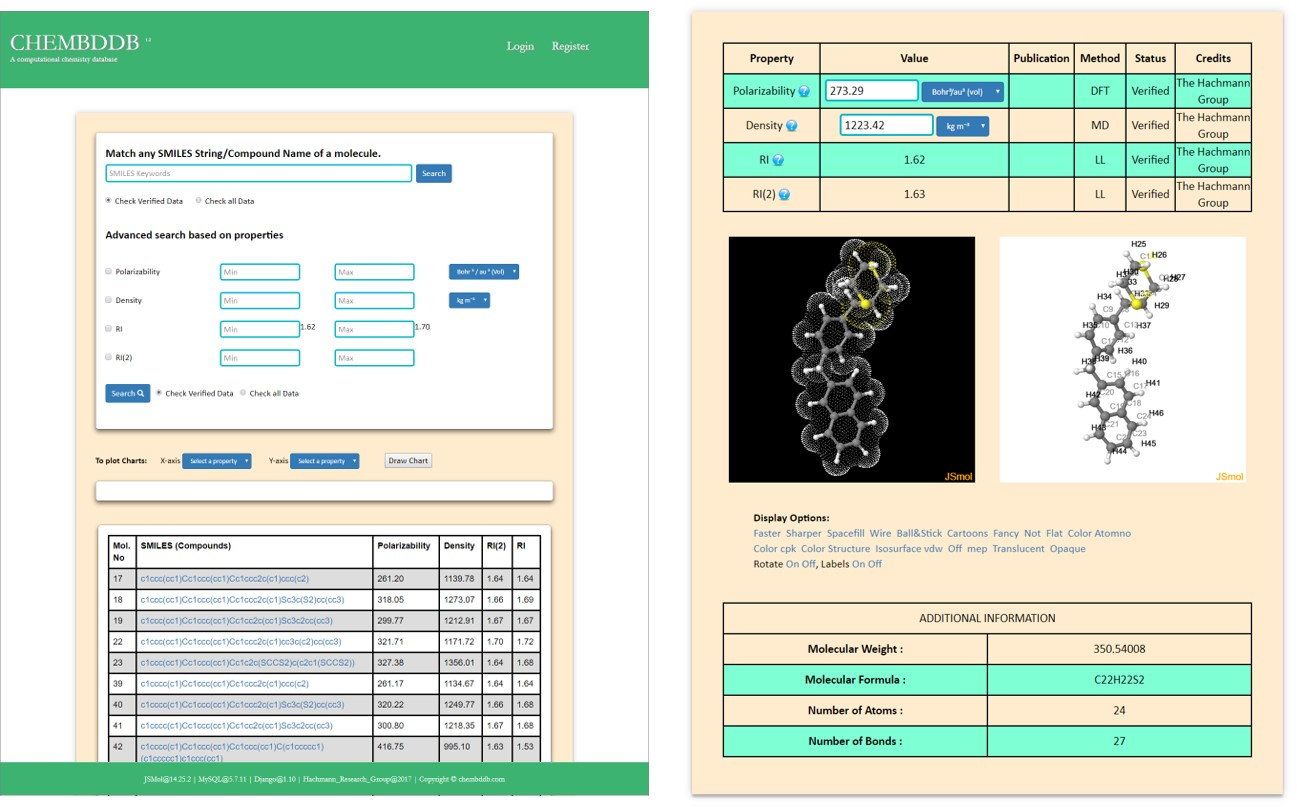
\includegraphics[width=1.0\textwidth]{Chapter-4/Figures/ChemBDDB_screeshot.jpg}
	\caption{Screenshots from the HRIP database.} 
	\label{fig:chembddb_screenshot} 
\end{figure}  

\subsection{Data Analysis, Mining, and Modeling Infrastructure}
\label{subsec:chemml}
We have been developing the \chemml\ program suite to establish data analysis, mining, and modeling capabilities that allow us to apply state-of-the-art machine learning and informatics methodology to chemical and materials data sets. \chemml 's principal tasks are the creation of predictive regression models and chemical pattern recognition/classification \cite{Kowalski1972}.

% introduce data-driven research; point to MGI and other high-profile initiatives for support of promise 
The resulting mapping functions (\ie  data-derived prediction models) are usually much easier to evaluate than physical models (\eg  the Schr\"odinger equation), so using them allows us to dramatically accelerate the characterization of chemical systems and it thus enables the hyperscreening of chemical space. 
A typical \chemml\ workflow encompasses a number of distinct steps that can be categorized in six main tasks: (1) input/output, (2) preprocessing, (3) learning, (4) validation, (5) evaluation, and (6) visualization. 

\chemml\ provides facilities for all these tasks \via\ classes of methods. These are either accessed from advanced third-party libraries and stand-alone programs (\eg  scikit-learn \cite{Pedregosa2011a}, Tensorflow \cite{tensorflow2015-whitepaper}, Keras \cite{chollet2015keras}, Dragon \cite{Taletesrl2011}, OpenBabel \cite{O'Boyle2011}, RDKit \cite{RDKit}), if these represent the state of the art for certain tasks, or from \chemmllib\ where we compile our new/original contributions as well as existing methods that are not otherwise accessible.  
The feature representation and the machine learning approach are two particularly important aspects in the generation of data-derived models, and they determine a model's predictive performance. 
\chemml\ can readily call many standard machine learning (as well as preprocessing and visualization) methods. Examples of available algorithms include multivariate regression \cite{ChristopherMBishop}, support vector machines \cite{Muller2001}, artificial neural networks \cite{Manzhos2006,Behler2007}, and deep learning \cite{dahl2015deep}. 
To support chemistry applications, \chemml\ interfaces the core learning algorithms with domain-specific tools, such as the feature space of molecular descriptors \cite{Todeschini2000,Sykora2008}, topological fingerprints \cite{Nilakantan1987,OBoyle2016c}, or more recent developments such as the Coulomb matrix \cite{Rupp2012} and bag-of-bonds \cite{Hansen2015b} descriptors. These feature spaces are the abstract `basis set' in terms of which a machine learning model for a particular structure-property relationship is numerically expressed \cite{Ramakrishnan2017}, and \chemml\ provides a comprehensive collection of existing schemes. While our current work focuses on supervised learning, we plan to broaden our scope to unsupervised and reinforcement learning in the future. 

The primary developer of \chemml\ is Mojtaba Haghighatlari. Other contributors include Ramachandran Subramanian, Bhargava Urala, Gaurav Vishwakarma, Aditya Sonpal, Po-Han Chen, and Srirangaraj Setlur.



\section{Software Ecosystem}
\label{subsec:ecosystem}
The four program packages discussed in the previous sections (\chemlg, \chemhtps, \chembddb, and \chemml) are loosely connected, \ie  they can either be employed as a comprehensive unit (see Fig.\ \ref{fig:ecosystem}), or in combination with drop-in replacements (\eg  with a different library generator or a custom database engine), or as standalone applications. 
The development work on our software ecosystem includes conceptual work, the design and assessment of protocols and workflows, the formulation of guidelines and best practices, and the implementation of both glue code and new methods. 
The key cyberinfrastructure challenges include the robust abstraction of workflows for general-purpose applications, scaling issues (\eg  associated with expensive data generation and the combinatorial nature of chemical space), code sustainability, as well as platform and distribution issues. While we emphasize black-box automation to reach non-expert users, we allow full customization of all settings (in particular in \chemml ). We continually extend and refine the features and capabilities of all four codes. These improvements are driven by feedback from application projects both inside and outside our group (cf.\ Sec.\ \ref{subsec:chemlg_app}). This input from different real-world application problems is a key to making this cyberinfrastructure as resourceful as possible. All codes are open and freely shared with the community under 3-clause BSD license \cite{Afzal2018b,Afzal2018c,Shirish2018,Haghighatlari2017}. All the repositories on GitHub are maintained by Hachmann Group. 

There are a number of exciting, high-profile software development efforts along similar lines by others in the field (\eg  \cite{Gunter2012,Ward2016}). 
% TODO: add better Materials Project reference and work by Kristin Persson; Open Chemistry
However, despite great popular demand, there is currently no cyberinfrastructure for data-driven \insilico\ research that is accessible to the community, applicable to a wide range of chemical problems, and that offers a level of comprehensiveness, automation, and integration comparable to that of modern computational chemistry program packages. Our contribution pursues this niche, which stands out in its scope and prospective utility.    

\section{Conclusions}

\label{sec:conclusions4}

The developed massively parallel generator, \chemlg, and the program suite for automated, virtual high-throughput screening studies, \chemhtps, offers a multitude of options to customize and restrict the scope of the enumerated chemical space and thus tailor it for the demands of specific applications. We incorporate genetic algorithms into the framework to streamline the non-combinatorial exploration of chemical space. Genetic algorithms have shown to be effective in optimizing chemical structures and generating useful compounds for different target applications. The parallel implementation of these codes and their integration with HPC systems allows us to create and setup screening of millions of molecular candidates in few seconds to minutes. 
	 
%Our software ecosystem recognizes the great opportunities that are arising with the shift towards a data-driven \insilico\ research paradigm in chemistry, materials science, and the corresponding engineering disciplines. 
%It focuses on delivering and deploying a cyberinfrastructure that is filling a distinct infrastructure gap and on building foundations that make data-driven research a viable and widely accessible proposition for the chemistry community. 
%The template for our efforts is the rise of computational chemistry program packages over the past decades and the tremendous impact it has had on the role of modeling and simulation in contemporary chemical research. 
%Following this example, our research program aims to advance our capacity to tackle complex discovery and design challenges, and improve our understanding of the associated molecular systems.
%We have shown in real-life application projects that this approach indeed offers a path to overcoming some of the prevalent limitations of traditional trial-and-error approaches. 


